\subsection{Krylov Subspace Methods}
\label{sec:krylov_methods}

Even though the methods introduced in the previous chapter are guaranteed to converge, the restriction to a one-dimensional search space severely limits their convergence behaviour. Since the error is only minimized along the current search direction, multiple iterations might actually end up optimizing along the same search space. Thus they might require a large number of iterations before they produce an accurate approximation of the desired solution. As a natural extension, faster progress could be expected from a larger search-space by minimizing the residual over multiple dimensions at the same time. Simultaneously, the search-space has to remain small enough in order to obtain a fast solution to the minimization process. Since there is a trade-off between the minimization cost and the number of iterations, an intuitive solution would be to create a sequence of subspaces $S$ with increasing dimensions such that:
\begin{equation}
    S_1 \subset \ S_2 \subset S_3 \subset \dots
\end{equation}

\noindent At each iteration $k$ of the iterative solver, the subspace $S_k$ satisfying $dim(S_k)=k$ is searched for a solution $\iter{x}$ that minimizes:
\begin{equation}
\label{eqn:residual}
    f(x)= r = Ax-b
\end{equation}

\noindent Note that because $S_n=\real$, this sequence will ultimately produce the exact solution to the problem (in absence of rounding errors). However, since this would amount to more work than just solving the system directly, a good approximation should be achieved in $k$ iterations with $k \ll n$. Hence, the challenge is to find such a subspace sequence that minimizes $r$ in the most optimal way. As illustrated in the one-dimensional case, the error of the approximation decreases most rapidly in the direction of the residual. Consequently it seems reasonable to choose $S_{k+1}$ at iteration $k$ so that it includes both $\iter[k]{x}$ and $\iter[k]{r}$, which guarantees that the update $\iter[k+1]{x}$ will be at least as good as the one-dimensional case \cite{golub_matrix_2013}. From $\iter[0]{x}$ as the initial guess and Equation~\hyperref[eqn:residual]{\ref{eqn:residual}} it follows that $\iter[k]{r} \in span\langle\iter[k]{x},A\iter[k]{x}\rangle$ and the only way to satisfy this requirement is:
\begin{equation}
    S_m=\mathcal{K}(A,\iter[0]{r}, m) = span\langle\iter[0]{r}, A\iter[0]{r}, A^2\iter[0]{r},\dots A^{m-1}\iter[0]{r}\rangle
\end{equation}

\noindent This kind of sequence is referred to as a Kryolov subspace and viewed from the angle of polynomial approximation, a vector $v$ in such a Krylov subspace can be expressed in general terms as a linear combination of powers of $A$ times $y$:
\begin{equation}
\label{eqn:poly1}
    v = c_0y+c_1Ay+c_2A^2y+\dots+c_{m-1}A^{m-1}y
\end{equation}

\noindent In other words $v$ is a polynomial in $A$ times $y$ and by defining $p$ as a polynomial of the form $p(z) = c_0+c_qz+c_2z^2+\dots+c_{m-1}z^{m-1}$, the following, compact description can be achieved:
\begin{equation}
\label{eqn:poly2}
v=p(A)y  
\end{equation}

\noindent A Krylov subspace method for solving a linear system will thus attempt to improve a initial solution $\iter[0]{x}$ based on the residual $\iter[0]{r} = b-A\iter[0]{x}$ by updating it with such a vector $v \in \mathcal{K}(A, \iter[0]{r},m)$, which corresponds to:
\begin{equation}
    A^{-1}b \approx \iter[m]{x} = \iter[0]{x}+p(A)\iter[0]{r}
\end{equation}

\noindent From this point going forward, $\mathcal{K}(A, \iter[0]{r},m)$ will be simply denoted as $\mathcal{K}_m$ if there is no ambiguity. Furthermore, note that even though all Krylov subspace based techniques provide the same type of polynomial approximation, they differ in the constraints $\mathcal{L}_m$ used to build these approximation, giving rise to a number of distinct algorithm (see \cite{saad_iterative_2003} for a comprehensive overview) and only a subset will be discussed in this research.



\subsubsection{Conjugate Gradient (CG)}
\label{sec:conjugate_gradient}

The easiest way to interpret the conjugated gradient method (first proposed by Hestenes \& Stiefel,  \cite{hestenes_methods_1952} is as an extension of the steepest descent algorithm to Krylov subspaces. Indeed, since in the first iteration, the Krylov subspace is defined as $\mathcal{K}_1=\{\iter[0]{r}\}$, the initial steps taken by the two algorithms are exactly equivalent. However, for CG the projection subspace extends in the second iteration to $\mathcal{K}_2=\{\iter[0]{r}, A\iter[0]{r}\}$ (a two-dimensional space), while it remains one dimensional for steepest descent. In other words, both methods optimize the error $\iter[0]{d}$ in the first step along the residual vector $\iter[0]{r}$ (i.e. the search direction $\iter[0]{p}=\iter[0]{r}$), but they differ in the second step. While steepest descent minimizes the new error $\iter[1]{d}$ only along the new residual $\iter[1]{r}$ (i.e. $\iter[1]{p}=\iter[1]{r}$), CG minimizes the error for the whole plane spanned by $span\langle\iter[0]{r}, \iter[1]{r}\rangle$. This can be achieved by selecting a new search direction $\iter[1]{p}$ that is $A$-orthogonal to all previous ones \cite{trefethen_numerical_1997}. If the bases of the Krylov subspace are rewritten as:
\begin{equation}
    \mathcal{K}_m = span\langle\iter[0]{r}, A\iter[0]{r}, \dots A^{m-1}\iter[0]{r}\rangle = span\langle\bm{q}_0, \bm{q}_1, \dots, \bm{q}_{m-1}\rangle
\end{equation}

\noindent Then, this corresponds to the condition $\bm{q}_i \perp \bm{q}_j$ with $i\neq j$ for all $i$,$j$ from $0$ to $m$. As a result, the algorithm introduced by \cite{hestenes_methods_1952} requires two modifications when compared to steepest descent.
\begin{enumerate}
    \item Introduce a vector $p$ ($\iter[0]{p} = \iter[0]{r}$) representing the search direction.
    \item Determine the new search direction $\iter[k+1]{p}$ so that it is $A$-orthogonal to all previous ones (or, equivalently, create an orthogonal basis $\bm{q}_{k}$ for the Krylov subspace $\mathcal{K}_{k+1}$).
\end{enumerate}

\begin{algorithm}[h]
  \caption{Conjugate Gradient}
  \label{alg:conjugate_gradient}
  \SetAlgoLined
  \DontPrintSemicolon
  \KwIn{matrix $A \in \mathbb{R}^{n \times n}$, vector $b \in \mathbb{R}^{n}$ and initial solution $\iter[0]{x} \in \mathbb{R}^{n}$}
  \KwOut{approximate solution $\iter[m]{x}$ to the system $Ax=b$\\
  \hrulealg}
  $\iter[0]{r} = b-A\iter[0]{x}$ \\
  $p = \iter[0]{r}$ \\
  \For{$k = 1$ \KwTo $m$} {
    $\alpha = \langle \iter[k-1]{r};\iter[k-1]{r} \rangle / \langle Ap;p \rangle$ \\
    $\iter{x} = \iter[k-1]{x}+\alpha p$ \\
    $\iter{r} = \iter[k-1]{r} - \alpha Ap$ \\
    $\beta = \langle \iter{r};\iter{r} \rangle / \langle \iter[k-1]{r};\iter[k-1]{r} \rangle$ \\
    $p = \iter{r} + \beta p$ \\
  }
\end{algorithm}

\noindent The pseudo-code provided in Algorithm~\hyperref[alg:conjugate_gradient]{\ref{alg:conjugate_gradient}} implements those changes. The modifications in line 4 correspond to the requierement that the new residual needs to be orthogonal to the Krylov subspace $\mathcal{K}_{k-1}$ (instead of just the previous residual), using a little simplification in the numerator of the fraction. Because $p$ is built as a linear combination of the previous residuals, $\langle \iter{r};\iter{r} \rangle = \langle \iter{r};\iter{p} \rangle$ is valid and the terms can be used interchangeably. The addition of lines 7 \& 8 corresponds to the Gram-Schmidt orthogonalization of the basis vectors, ensuring that the new search direction is $A$-orthogonal to all previous ones. Note that since $\iter[k]{p}$ is already $A$-orthogonal to all $\iter[i]{p}, i=0,\dots,k-1$, the only orthogonalization that is needed for $\iter[k+1]{p}$ is with respect to $\iter[k]{p}$. In other words, we have the following identities of subspaces:
\begin{equation}
  \begin{aligned}
    \mathcal{K}_m 
    & =\langle \iter[1]{x}, \iter[2]{x}, \dots \iter[m]{x} \rangle 
   & & = \langle \iter[0]{p}, \iter[1]{p}, \dots \iter[m-1]{p} \rangle \\
    & = \langle \iter[0]{r}, \iter[1]{r}, \dots \iter[m-1]{r} \rangle
   & & =\langle \iter[0]{r}, A\iter[0]{r}, \dots A^{m-1}\iter[0]{r}\rangle\\
  \end{aligned}
\end{equation}

\noindent Furthermore, for those subspaces, the following properties hold:
\begin{equation}
    \langle\iter[i]{r};\iter[j]{r}\rangle =0 \;\; \text{ and } \;\; \langle\iter[i]{p};\iter[j]{p}\rangle_A =0
    \;\; \text{ for all }\;\; i,j <m, i \neq j
\end{equation}

\noindent Since all Krylov subspace iterations can be analyzed in terms of matrix polynomials (see Equations~\hyperref[eqn:poly1]{\ref{eqn:poly1}} \& \hyperref[eqn:poly2]{\ref{eqn:poly2}}), the same is true for the CG method. By defining $P_k$ as the set of polynomials $q$ of degree $\leq m$ with $q(0)=1$ and $\iter[0]{d}$ denoting the initial error $\iter[0]{d} = x^*-\iter[0]{x}$ the problem CG tries to solve can be reformulated as finding the polynomial $q_m$ such that:
\begin{equation}
\label{eqn:cg_poly}
    p_m = \underset{p\in P_m}{min} \norm{p_m(A)\iter[0]{d}}_A
\end{equation}

\noindent In terms of convergence of the CG method, it is known that the speed depends on the location of the spectrum of $A$ and \cite{trefethen_numerical_1997} expressed the two best known corollaries in the following form:
\begin{itemize}
    \item CG converges in at most $m$ steps, if $A$ has exactly $m$ distinct eigenvalues
    \item If the condition number $\kappa_2(A) $ is not too large, convergence can be expected in $\mathcal{O}(\sqrt{\kappa_2(A})$ iterations because the following is known for the error $d$:
\begin{equation}
        \frac{\norm{\iter[m]{d}}_A}{\norm{\iter[0]{d}}_A} \leq 2 \left( \frac{\sqrt{\kappa_2(A)}-1}{\sqrt{\kappa_2(A)}+1}\right)^m
\end{equation}
\end{itemize}

\noindent Finally, it should be noted that the formulation in Algorithm~\hyperref[alg:conjugate_gradient]{\ref{alg:conjugate_gradient}} is the one originally proposed by \cite{hestenes_methods_1952}, but several other alternative variants are possible (for example based on the Lanczos iteration, see Section~\hyperref[sec:lanczos]{\ref{sec:lanczos}}). The key point is the construction of the orthogonal bases for the Krylov subspace $\mathcal{K}_m$ and, depending on how those are obtained (e.g. the orthogonalization scheme employed), the denotations of the algorithms deviate slightly. Due to the importance of this part for all Krylov subspace based iterative methods, the two main techniques for obtaining such bases will be discussed in the next sections.


\subsubsection{Arnolid's method}
\label{sec:arnoldi}
This method, first proposed by Arnoldi \cite{arnoldi_principle_1951} enforces the Galerkin condition $A\iter[k]{x} -b \perp \mathcal{K}_k$ onto the constructed Krylov subspace and is applicable to general non-symmetric matrices. It was originally proposed for the purpose of reducing a dense matrix into Hessenberg from via a unitary transformation. But at its core, it is an algorithm for building an orthogonal basis of the Krylov subspace $\mathcal{K}_k$. It was later discovered that it is also an efficient technique for eigenvalue approximation, and was then extended to the solution of linear systems \cite{saad_iterative_2003}. 

\begin{algorithm}[h]
  \caption{Arnoldi's Method}
  \label{alg:arnoldi}
  \SetAlgoLined
  \KwIn{non-singular matrix $A \in \mathbb{R}^{n \times n}$, arbitrary vector $y \in \mathbb{R}^{n}$}
  \KwOut{\\ Hessenberg matrix $H \in \mathbb{R}^{(m+1) \times m}$ \\
  sequence of orthonormal vectors $\iter[i]{q}\in \mathbb{R}^{n}$ where $i = 1, 2, \dots, k$\\
  \hrulealg}
  $\iter[1]{q}= y\:/\norm{y}_2$ \\
  \For{$i = 1$ \KwTo $k$} {
    $w =A\cdot \iter[i]{q}$ \\
    \For{$j = 1$ \KwTo $i$} {
      $h_{j,i} = w^T\cdot \iter[j]{q}$ \\
      $ w = w - h_{j,i}\cdot \iter[j]{q}$}
    $h_{i-1,i} = \norm{w}_2$ \\
    \If{$h_{i-1,i} = 0$}{\Return}
    $\iter[i-1]{q} = w/h_{i+1,i}$
  }
\end{algorithm}

\noindent Following the process outlined in Algorithm~\hyperref[alg:arnoldi]{\ref{alg:arnoldi}}, the successive iterates are related by the following formula:
\begin{equation}
\label{eqn:arnoldi}
AQ_k=Q_{k+1}\tilde{H}_k
\end{equation}
\noindent where $\tilde{H}_k$ is the $(k+1) \times k$ upper-left section of $H$ (and thus also a Hessenberg matrix) and $Q_k$ is:
\begin{equation}
  Q_k =
  \left[
    \begin{array}{c|c|c}
      & & \\
      \iter[1]{q} &\dots & \iter[k]{q} \\
      & & \\
    \end{array}
  \right] 
\end{equation}

\noindent This is equivalent to:

\begin{equation}
  \left[
    \begin{array}{ccc}
      &  & \\
      & A & \\
      &  & \\
    \end{array}
  \right] \cdot
  \left[
    \begin{array}{c|c|c}
      & & \\
      \iter[1]{q} &\dots & \iter[k]{q} \\
      & & \\
    \end{array}
  \right] = 
  \left[
    \begin{array}{c|c|c}
      & & \\
      \iter[1]{q} &\dots & \iter[k+1]{q} \\
      & & \\
    \end{array}
  \right]
  \left[
    \begin{array}{ccc}
      h_{1,1} & \dots & h_{1,k} \\
      h_{2,1} & \dots &  h_{2,k}\\
      & \ddots & \vdots \\
      & & h_{k+1, k}  \\
    \end{array}
  \right] 
\end{equation}

\noindent Therefore, the $k$-th column of this equation can be denoted as:
\begin{equation}
    A \cdot \iter[k]{q} = h_{1,k}\cdot \iter[1]{q}+ \cdots + h_{k,k}\cdot \iter[k]{q} + h_{k+1,k}\cdot \iter[k+1]{q}
\end{equation}

\noindent From this, it is evident that the vectors $q^i$ form orthonormal bases of the successive Krylov subspaces generated by $A$ and $y$:
\begin{equation}
\label{eqn:krylov_space}
    \mathcal{K}_k=\langle y, Ay, \dots , A^{k-1}y\rangle = \langle \iter[1]{q},\iter[2]{q}, \dots , \iter[k]{q}\rangle
\end{equation}

\noindent Expressed in terms of matrix polynomials, Arnolid's method can also be analyzed by defining

Since Krylov subspace iterations can be analyzed in terms of matrix polynomials (see Equations~\hyperref[eqn:poly1]{\ref{eqn:poly1}} \& \hyperref[eqn:poly2]{\ref{eqn:poly2}}), the same is true for Arnoldi's method. By defining 
\begin{equation}
\label{eqn:arnoldi_poly}
    P^k = \{\text{monic polynomials of degree }k\}\text{,}
\end{equation}

\noindent  That is $P^k$ refers to all polynomials where the coefficient of the term of degree $k$ (note that a superscript is used instead of a subscript to differentiate this case from the CG analysis in Equations~\hyperref[eqn:cg_poly]{\ref{eqn:cg_poly}}). If $p \ in P^k$ the vector from Equation~\hyperref[eqn:poly2]{\ref{eqn:poly2}} can be written as $p^k(A)y=A^ky-Q_kz$ for some $z \in \mathbb{R}^k$. The orthogonality condition can be rewritten as $p^k(A)y \perp \mathcal{K}_m$ and hence Arnoldi's method has the remarkable property that it finds $z$ such that $\norm{A^ky-Q_kz}_2$ is minimal. In other words, it solves the least squares polynomial approximation problem:
\begin{equation}
\label{eqn:poly_arnoldi}
    \norm{p^k(A)y}_2 = \text{ minimum}
\end{equation}
\noindent The full proof behind this characteristic can be obtained from \cite{trefethen_numerical_1997}, but the general intuition is analogous to the case of an orthogonal projection and illustrated in Figure~\hyperref[fig:arnoldi]{\ref{fig:arnoldi}}.

\begin{figure}[h]
    \centering
    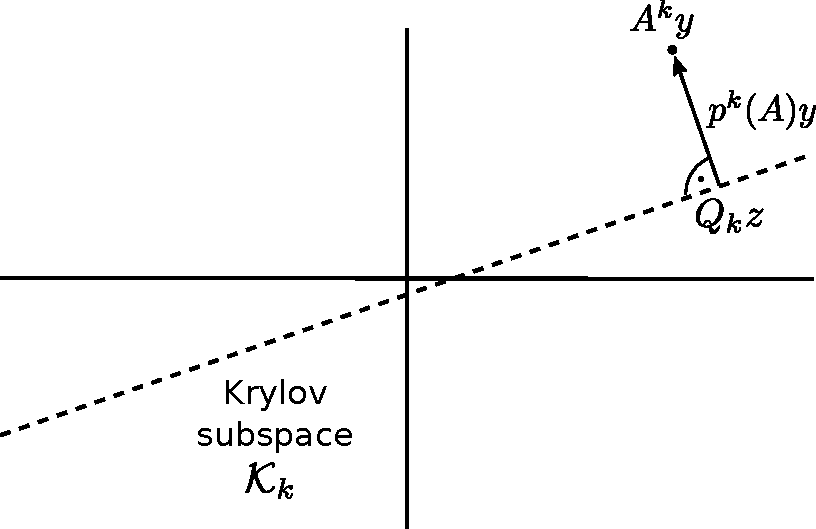
\includegraphics[width=0.6\linewidth]{chapters/3_solvers/3_2_iterative_solvers/figures/Arnoldi.pdf}
    \caption{The least squares polynomial approximation problem underlying the Arnoldi iteration as described in \cite{trefethen_numerical_1997}.}
    \label{fig:arnoldi}
\end{figure}

\noindent A final remark on Arnoldi's method has to be made with regards to numerical stability. As can be seen from the pseudo-code given in Algorithm~\hyperref[alg:arnoldi]{\ref{alg:arnoldi}}, the method needs to orthonormalize the resulting vector $w$ against all previous $\iter[j]{q}$'s in each iteration. While several methods are known to achieve this outcome, they differ in terms of speed and numerical stability (for a discussion of the different methods, see \cite{golub_matrix_2013} or \cite{trefethen_numerical_1997}). Algorithm~\hyperref[alg:arnoldi]{\ref{alg:arnoldi}} used the Modified-Gram-Schmidt method, but in principle, any other orthonormalization technique can be incorporated into the process. Pseudo-code for variants using ordinary Gram-Schmidt or Householder orthogonalization can be obtained from \cite{saad_iterative_2003}.


\subsubsection{The Lanczos Iteration}
\label{sec:lanczos}

The Lanczos algorithm can by viewed as a specialization of Arnoldi's method that focuses on the symmetric case. The first observation that needs to be made is that, if Arnoldi's method is applied to a symmetric matrix $A$, it will result in a tridiagonal, symmetric Hessenberg matrix $A$ \cite{saad_gmres_1986}. Hence the inner iterations of the nested loop in Algorithm~\hyperref[alg:arnoldi]{\ref{alg:arnoldi}} becomes much cheaper to compute since $h_{i,j} = 0$ for $1 \leq i < j-1$. This property is relatively simple to proof. In general a single entry of the matrix $H$ is given by:
\begin{equation}
    h_{i,j}=q^{(i)T} A\iter[j]{q}
\end{equation}

\noindent Because $A\iter[i]{q} \in \langle \iter[1]{q},\iter[2]{q}, \dots , \iter[k]{q}\rangle $, this implies that $h_{i,j} = 0$ for $i>j+1$ since the Krylov vectors are orthogonal. By taking the transpose of this formula one obtains:
\begin{equation}
        h_{i,j}=q^{(j)T} A\iter[i]{q}
\end{equation}

\noindent In the symmetric case $\transp{A} = A$ and $h_{i,j} = 0$ for $j>i+1$ following the same reasoning as before. In the standard notation for the Lanczos iteration $T_k$ denotes the resulting matrix $H_k$, which takes the following form (as given in \cite{trefethen_numerical_1997}):
\begin{equation}
\label{eqn:lanczos}
   T_k = \left[
    \begin{array}{ccccc}
      \alpha_1 & \beta_1 & & & \\
      \beta_1 & \alpha_2 & \beta_2  & & \\
      & \beta_2 & \alpha_3 & \ddots  & \\
       & &\ddots &\ddots &\beta_{k-1} \\
       & & &\beta_{k-1} &\alpha_{k} \\
    \end{array}
  \right] 
\end{equation}

\noindent Following this notation, Algorithm~\hyperref[alg:arnoldi]{\ref{alg:arnoldi}} illustrates the Lanczos process in pseudo-code. Compared to Arnoli's method it consists of only a single loop, but otherwise guarantees the exact same properties. It solves the exact same optimization problem (in Equation~\hyperref[eqn:poly_arnoldi]{\ref{eqn:poly_arnoldi}}) and is much more preferable in terms of algorithmic and storage complexity given that the matrix $A$ is symmetric. 

\begin{algorithm}[h]
  \caption{The Lanczos Iteration}
  \label{alg:lanczos}
  \SetAlgoLined
  \KwIn{non-singular symmetric matrix $A \in \mathbb{R}^{n \times n}$, arbitrary vector $y \in \mathbb{R}^{n}$}
  \KwOut{\\ tridiagonal symmetric matrix $T \in \mathbb{R}^{(m+1) \times m}$ \\
  sequence of orthonormal vectors $\iter[i]{q}\in \mathbb{R}^{n}$ where $i = 1, 2, \dots, k$\\
  \hrulealg}
  $\beta_0= \iter[0]{q} =0 $\\
  $\iter[1]{q}= y\:/\norm{y}_2$ \\
  \For{$i = 1$ \KwTo $k$} {
    $w =A\cdot \iter[i]{q}$ \\
    $\alpha_i = q^{(i)T}\cdot w$ \\
    $w = w -\beta_{i-1}\iter[i-1]{q}-\alpha_i\iter[i]{q}$ \\
    $\beta_i = \norm{w}_2$ \\
     \If{$\beta_i = 0$}{\Return} 
    $\iter[i+1]{q} = w/\beta_i$
  }
\end{algorithm}

However, the Lanczos iteration guarantees orthogonality of the resulting Krylov vectors in exact arithmetic only. Because of the limits of floating-point calculations, \cite{saad_gmres_1986} states that exact orthogonality of these vectors can only be observed in the beginning of the iteration. Due to the accumulation of rounding-errors the vectors will start to lose their global orthogonality property at some point (and decay rapidly), posing a serious obstacle for iterative solvers. Therefore, multiple schemes to account for lost orthogonality by recovering or diminishing its effects have been developed (see \cite{parlett_beresford_n_13_1998}).

\subsubsection{Minimal Residual Method (MINRES)}
\label{sec:minres}
The minimal residual method (MINRES) has been developed by \cite{paige_solution_1975} as an extension of the CG method based on the Lanczos iteration in order to solve symmetric indefinite linear systems. It is motivated by the fact that the CG formulation of \cite{hestenes_methods_1952} can be derived from the Cholesky factorization of the matrix $T_k$ created by the Lanczos process. Since the Cholesky factorization requires the matrix $T_k$ to be positive definite (which is the case if $A$ is positive definite, see \cite{paige_solution_1975}), the key idea is to use a factorization technique without this requirement. If for example, the LU factorization is used, the decomposition would take the following form:
\begin{equation}
       T_k = L_k U_k=
  \left[
    \begin{array}{ccccc}
      1 &  & & & \\
      \lambda_1 & 1 &  & & \\
      & \lambda_2 & 1 &  & \\
       & &\ddots &\ddots & \\
       & & &\lambda_{k-1} &1 \\
    \end{array}
  \right] 
  \left[
    \begin{array}{ccccc}
      \mu_1 & \beta_1 & & & \\
       & \mu_2 & \beta_2  & & \\
      &  & \mu_3 & \ddots  & \\
       & & &\ddots &\beta_{k-1} \\
       & & & &\mu_{k} \\
    \end{array}
  \right] 
\end{equation}

\noindent Note that in this factorization $\beta$ remains unchanged from the Lanczos process, while both $\lambda$ and $\mu$ result from the Gaussian elimination. They can be obtained via the following formulas:
\begin{equation}
    \begin{aligned}
    \mu_1 &= \alpha_1\\
    \lambda_k &= \frac{\beta_k}{\mu_{k}} \\
      \mu_k & = \alpha_k-\lambda_{k-1}\beta_{k-1}
    \end{aligned}
\end{equation}

\noindent The approximate solution for the $k$-th Krylov subspace is then given by (where $Q$ and $\beta$ are created by the Lanczos process):
\begin{equation}
    x_k = x_0 + Q_kU_k^{-1}L_k^{-1}(\beta e_1)
\end{equation}

\noindent This can then be used as an alternative formulation of the CG algorithm (although it should be noted that the previous formulation by \cite{hestenes_methods_1952} performs better in terms of storage and computing complexity). The pseudo-code for this version of the algorithm as well as the full derivation and proof of equality can be obtained from \cite{saad_iterative_2003}. However, if Gaussian elimination without pivoting is used, this algorithm is susceptible to breakdown. In \cite{paige_solution_1975}, the LQ factorization is suggested instead, giving rise to an algorithm named SYMMLQ, that can be used for indefinite symmetric problems. Unfortunately, as the main drawback of this proposal the $A$-norm of the error is no longer minimized, which can lead to a non-monotonic convergence. Therefore, in the same paper \cite{paige_solution_1975}, an extension called MINRES was proposed, that, as the name suggest, minimizes the norm of the residual instead.

Similar to how SYMMLQ is an extension of CG, MINRES has its equivalent for the symmetric positive case in the Conjugate Residual (CR) method illustrated in Algorithm~\hyperref[alg:conjugate_residual]{\ref{alg:conjugate_residual}}. As demonstrated on the example of steepest descent and MR in Section~\hyperref[sec:subspace_methods]{\ref{sec:subspace_methods}} those methods differ in the orthogonality condition employed, thus resulting in a different projection. As such, MR, CR and MINRES all optimize the norm of the residual in each iterations.


\begin{algorithm}[h]
  \caption{Conjugate Residual}
  \label{alg:conjugate_residual}
  \SetAlgoLined
  \DontPrintSemicolon
  \KwIn{matrix $A \in \mathbb{R}^{n \times n}$, vector $b \in \mathbb{R}^{n}$ and initial solution $\iter[0]{x} \in \mathbb{R}^{n}$}
  \KwOut{approximate solution $\iter[k]{x}$ to the system $Ax=b$\\
  \hrulealg}
  $\iter[0]{r} = b-A\iter[0]{x}$ \\
  $\iter[0]{p} = \iter[0]{r}$ \\
  \For{$i = 1$ \KwTo $k$} {
    $\alpha = \langle \iter[i-1]{r};A\iter[i-1]{r} \rangle / \langle A\iter[i-1]{p};A\iter[i-1]{p} \rangle$ \\
    $\iter[i]{x} = \iter[i-1]{x}+\alpha \iter[i-1]{p}$ \\
    $\iter[i]{r} = \iter[i-1]{r} - \alpha A\iter[i-1]{p}$ \\
    $\beta = \langle \iter[i]{r};A\iter[i]{r} \rangle / \langle \iter[i-1]{r};A\iter[i-1]{r} \rangle$ \\
    $\iter[i]{p} = \iter[i]{r} + \beta \iter[i-1]{p}$ \\
    \% optional optimization to avoid computing $A\iter[i]{p}$ multiple times \\
    $A\iter[i]{p} = A\iter[i]{r}+\beta A\iter[i-1]{p}$
  }
\end{algorithm}

MINRES now considers a QR factorization of the matrix $T_k$ (resulting from the $k$-th Lanczos iteration step), which takes the form:
\begin{equation}
    T_k= Q_k R_k \;\; \text{ with } \;\; Q_k \in \mathbb{R}^{(k+1)\times (k+1)}\;\; \text{ and } \;\; R_k \in \real[k]
\end{equation}

\noindent Note that it is not necessary to compute this decomposition at each step, since it can be computed from the previous one via Givens rotations (see Section %TODO)
In this decomposition, $R_k$ will have an upper triangular banded structure and it can be shown that minimizing the residual $\iter[k]{r}$ over the Krylov subspace $\mathcal{K}_k$ is equivalent to finding $\lambda_k$ such that (in the following, the matrix $Q_k$ obtained from the Lanczos iteration will be denoted as $V_k$ in order to avoid confusion):
\begin{equation}
    \transp{V_k}A^2V_k\lambda_k = \transp{V_k}Ab
\end{equation}

\noindent This can be rewritten as:
\begin{equation}
    \transp{T_k}T_k\lambda_k=\transp{T_k}\transp{V_{k+1}}b = \transp{T_k}\left[
        \begin{array}{c}
      \norm{b}_2 \\
       0 \\
      \vdots \\
      0 \\
    \end{array}\right]
\end{equation}

\noindent Making use of the QR-factorization this leads to:
\begin{equation}
    \transp{R_k}R_k\lambda_k=\transp{R_k}\transp{Q_{k}}\left[
        \begin{array}{c}
      \norm{b}_2 \\
       0 \\
      \vdots \\
      0 \\
    \end{array}\right]
\end{equation}

\noindent Which can alternatively be written as:
\begin{equation}
    R_k\lambda_k=I_k\transp{Q_{k}}\left[
        \begin{array}{c}
      \norm{b}_2 \\
       0 \\
      \vdots \\
      0 \\
    \end{array}\right]
\end{equation}

\noindent Because $R_k$ is guaranteed to be invertible in practice as long as $A$ is non-singular, this equation can be solved for $\lambda_k$ and the approximate solution for MINRES is obtained via:
\begin{equation}
    \iter[k]{x} = Q_k\lambda_k=Q_kR_k^{-1}R\lambda_k
\end{equation}



\subsubsection{Generalized Minimal Residuals (GMRES)}
\label{sec:gmres}

The generalized minimal residuals (GMRES) method can be viewed as an extension of MINRES for the non-symmetric case, using Arnoldi's method instead of the Lanczos iteration. It is due to \cite{saad_gmres_1986} and can be used in order to obtain a solution for general linear systems. The idea of this approach is simple: In every iteration $k$, the accurate solution is approximated by the vector $\iter[k]{x} \in \mathcal{K}_k$ such that it minimizes the norm of the residual $\iter[k]{x}=b-A\iter[k]{x}$. Or, if expressed as a polynomial approximation problem, it is defined as (and solves the same problem as the CR method):
\begin{equation}
    \iter[k]{r}=p_kA(y)
\end{equation}

\noindent Note that in contrast to Equation~\hyperref[eqn:arnoldi_poly]{\ref{eqn:arnoldi_poly}}, for Arnoldi's method, $p_k \in P_k$ where
\begin{equation}
    P_k = \{\text{polynomials } p \text{ of degree } \leq k \text{ with }p(0)=1\}
\end{equation}

\noindent This is the same definition as for the CG method and as such, a subscript is used again to denote this difference. The orthogonality condition is now $p_k(A)y \perp A\mathcal{K}_k$ as illustrated in Figure~\hyperref[fig:gmres]{\ref{fig:gmres}}. In matrix form this is equivalent to defining a Krylov matrix $K_k \in \mathbb{R}^{n \times k}$ which satisfies:
\begin{equation}
\label{eqn:krylov_matrix}
  AK_k =
  \left[
    \begin{array}{c|c|c|c}
      & & & \\
      Ab & A^2b & \dots & A^kb \\
      & & & \\
    \end{array}
  \right] 
\end{equation}

\begin{figure}[h]
    \centering
    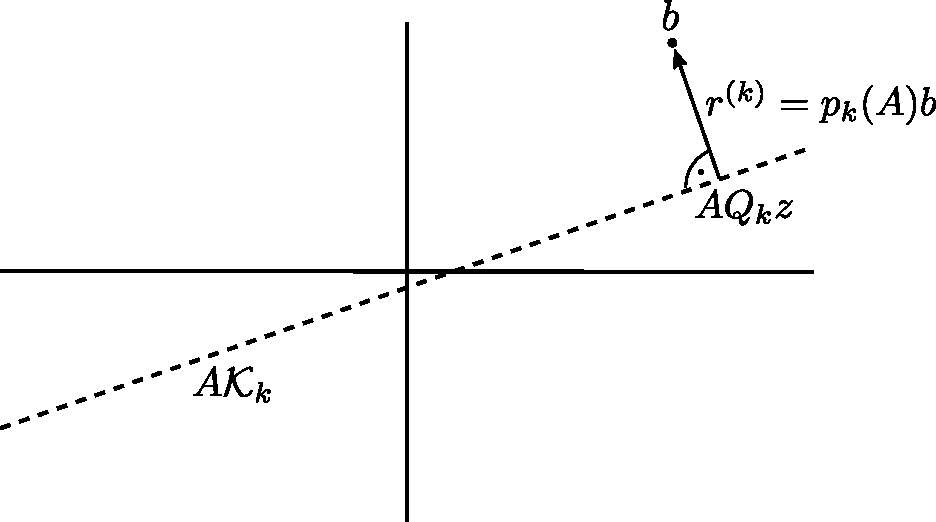
\includegraphics[width=0.7\linewidth]{chapters/3_solvers/3_2_iterative_solvers/figures/GMRES.pdf}
    \caption{The least squares polynomial approximation problem underlying the GMRES (minimizing $\norm{\iter[k]{r}}_2$), as described in \cite{trefethen_numerical_1997}}.
    \label{fig:gmres}
\end{figure}

\noindent From this, it is evident that the column space of that matrix is $A\mathcal{K}_k$ and the problem is reduced to finding a vector $c \in \mathbb{R}^{k}$ such that $\norm{AK_kc-b}_2$ is minimal   \cite{trefethen_numerical_1997}. Once this vector is obtained, the approximate solution would be given by $\iter[k]{x} =K_kc$. Solving the least squares problem could be achieved by computing a QR factorization of $AK_k$, but this procedure would be numerically unstable, since $K_k$ is exceedingly ill-conditioned \cite{trefethen_numerical_1997}. Instead, Arnoldi's method is used to construct a sequence of Krylov matrices $Q_k$ (spanning the successive Krylov subspaces $\mathcal{K}_k$) and then setting the approximate solution to $\iter[k]{x} = Q_ky$. Hence the problem can be reformulated as finding a vector $y \in \mathbb{R}^k$ satisfying:
\begin{equation}
    \norm{AQ_ky-b}_2=\text{ minimum}
\end{equation}

\noindent Using Equation~\hyperref[eqn:arnoldi]{\ref{eqn:arnoldi}} we obtain:
\begin{equation}
    \norm{Q_{k-1}\tilde{H}_k-b}_2=\text{ minimum}
\end{equation}

\noindent Now, multiplying by $Q^T_{k-1}$ from the left (which does not change the norm since both vectors are within the column space of $Q_{k-1}$), this is equivalent to:
\begin{equation}
    \norm{\tilde{H}_ky-Q^T_{k-1}b}_2 = \text{ minimum}
\end{equation}

\noindent From the construction of the Krylov matrices $\{Q_k\}$ (Equations~\hyperref[eqn:krylov_space]{\ref{eqn:krylov_space}} \& \hyperref[eqn:krylov_matrix]{\ref{eqn:krylov_matrix}}) it follows that $q_1=b\:/\norm{b}_2$ and $q_i \perp b$, for $i = 2, \dots, k+1$. Therefore, $Q^T_{k+1}b$ is equal to $\norm{b}_2e_1$, where $e_1=(1,0,0,\dots)^T$ and the solution to the GMRES least squares problem can be obtained by:
\begin{equation}
    \norm{\tilde{H}_ky-\norm{b}_2e_1}_2 = \text{ minimum}
\end{equation}

\noindent Due to the Hessenberg structure of $\tilde{H}_k$, this equation can be solved for $y$ via QR factorization at a reduced cost of $\mathcal{O}(k^2)$. Consequently GMRES is able to deliver a much faster solution than direct factorization, as long as the number of iterations $k$ remains small.

\begin{algorithm}[h]
  \caption{GMRES}
  \label{alg:gmres}
  \SetAlgoLined
  \DontPrintSemicolon
  \KwIn{non-singular matrix $A \in \mathbb{R}^{n \times n}$, vector $b \in \mathbb{R}^{n}$}
  \KwOut{approximate solution $\iter[k]{x}$ to the system $Ax=b$\\
  \hrulealg}
  $q_1= b\:/\norm{b}_2$ \\
  \% Arnoldi's method \\
  \For{$i = 1$ \KwTo $m$} {
    $w =A\cdot q^i$ \\
    \For{$j = 1$ \KwTo $i$} {
      $h_{j,i} = w^T\cdot q_j$ \\
      $ w = w - h_{j,i}\cdot q_j$}
    $h_{i-1,i} = \norm{w}_2$ \\
    \If{$h_{i-1,i} = 0$}{\Return $\iter[i]{x}$}
    $q_{i+1} = w/h_{i+1,i}$ \\
  }
  \;
  \% GMRES extension \\
  define $\tilde{H}_k = \{h_{i,j}\}, 1 \leq i \leq k+1, 1 \leq j \leq k$ \\
  define $Q_k = \{q_1, \cdots, q_k\}$ \\
  Find $y$ to minimize $\normd{\tilde{H}_ky-\norm{b}_2e_1}_2$ ($=\norm{\iter[k]{r}}_2$) \\
  $\iter[k]{x} = Q_ky$
\end{algorithm}

\noindent Algorithm~\hyperref[alg:gmres]{\ref{alg:gmres}} describes the general outline of the GMRES algorithm as provided by \cite{trefethen_numerical_1997} (based on Modified-Gram-Schmidt Arnoldi). From this, it is immediately evident that both storage and computational complexity are dependent on the number of iterations required. The original formulation of the algorithm \cite{saad_gmres_1986} differs slightly from the one given above, taking the residual as the starting vector for the iteration and solving the equation in line 18 for a correction term instead. This enables the method to be restarted from the current approximate solution after a certain number of iterations, preventing $k$ from growing prohibitively large. The required changes are illustrated in Algorithm~\hyperref[alg:gmres2]{\ref{alg:gmres2}}

\begin{algorithm}[h]
  \caption{GMRES (initial solution based)}
  \label{alg:gmres2}
  \SetAlgoLined
  \DontPrintSemicolon
  \KwIn{non-singular matrix $A \in \mathbb{R}^{n \times n}$, vector $b \in \mathbb{R}^{n}$, initial solution $\iter[0]{x} \in \mathbb{R}^{n}$}
  \KwOut{approximate solution $\iter[k]{x}$ to the system $Ax=b$\\
  \hrulealg}
  $\iter[0]{r} = b-A\iter[0]{x}$ \\
  $\beta = \norm{\iter[0]{r}}_2$ \\
  $q_1 = \iter[0]{r}/\beta$ \\
  \For{$i = 1$ \KwTo $k$} {
   $\langle$ step $i$ of Arnoldi's method (e.g. Algorithm~\hyperref[alg:arnoldi]{\ref{alg:arnoldi}} $\rangle$ \\
  }
  define $\tilde{H}_m = \{h_{i,j}\}, 1 \leq i \leq k+1, 1 \leq j \leq k$ \\
  define $Q_k = \{q_1, \cdots, q_k\}$ \\
  Find $y$ to minimize $\normd{\tilde{H}_ky-\beta e_1}_2$ \\
  $\iter[k]{x} = \iter[0]{x}Q_ky$
\end{algorithm}

A disadvantage of both variants of the algorithm is that they do not provide the approximate solution $\iter[k]{x}$ at each step and it is therefore difficult to determine how many iterations are needed. However, this issue can be alleviated by using plane rotations to transform the Hessenberg matrix into upper triangular form. Since this is a common technique for solving the problem $min(\normd{\tilde{H}_ky-\beta e_1}_2)$, it can basically be performed at zero additional cost. By defining a sequence of rotations matrices $\Omega_i \in \mathbb{R}^{(k+1) \times (k+1)}$ of the form:
\begin{equation}
    \Omega_i=
    \begin{blockarray}{*{8}{c} l}
    \begin{block}{[*{8}{c}] l}
      1 & & & & & & & \\
      & \ddots & & & & & & \\
      & & 1 & & & & & \\
      & & &c_i & s_i& & &  \bigstrut[t] & \leftarrow \text{row } i\\
      & & &-s_i & c_i& & & \bigstrut[t] & \leftarrow \text{row } i+1\\
      & & & & & 1& & \\
      & & & & & & \ddots & \\
      & & & & & & & 1\\
    \end{block}
    \end{blockarray}
\end{equation}

\noindent Note that $s_i$ and $c_i$ are scalars satisfying $c^2_i+s^2_i=1$ and can generally be obtained via the formulas given in \cite{saad_iterative_2003}:
\begin{equation}
    s_i=\frac{h_{i+1, i}}{\sqrt{(h^{(i-1}_{i,i}=^2+h^2_{i+1, i}}}\text{,   } \;\;c_i=\frac{h^{(i-1)}_{i+1, i}}{\sqrt{(h^{(i-1}_{i,i}=^2+h^2_{i+1, i}}}
\end{equation}

\noindent By defining $V_k$ as the product of the rotation matrices $\Omega_i$
\begin{equation}
    V_k = \Omega_k \Omega_{k-1} \dots \Omega_1
\end{equation}
\noindent and
\begin{equation}
    \tilde{R}_k = V_k\tilde{H}_k 
\end{equation}
\begin{equation}
        \tilde{g}_k = V_k(\beta e_1) = (\gamma_1, \cdots, \gamma_{k+1})^T
\end{equation}

\noindent Thus, the problem can be reformulated as $min(\normd{\beta e_1 -\tilde{H}_ky}_2==min(\normd{\tilde{g}_k -\tilde{R}_ky}_2)$, thanks to $V_k$ being unitary. A detailed proof for this equation is given in \cite{saad_iterative_2003}. The big advantage of this method is not only that $\tilde{R}_k$ is triangular (and hence easily solvable), but also that the current residual (i.e. at step $k$) is readily available as $\gamma_{k+1}$.

Having obtained a satisfactory criterion to determine convergence, it is natural to ask for the upper bound of the number of iterations required by GMRES. Following the analysis in \cite{trefethen_numerical_1997}, we can observe that the algorithm converges monotonically, since $\norm{\iter[k]{r}}_2$ is minimal for the subspace $\mathcal{K}_k$, it can only decrease (or, at worst remain unchanged) by enlarging the space to $\mathcal{K}_{k+1}$.
\begin{equation}
    \norm{\iter[k-1]{r}}_2\leq \norm{\iter[k]{r}}_2
\end{equation}

\noindent Secondly, after at most $k$ steps, the process must converge in the absence of rounding errors and $\norm{\iter[k]{r}}_2 = 0$. However, to be useful as an iterative method, satisfactory accuracy must be achieved with  $k \ll n$. Expressed in terms of polynomial approximation: 
\begin{equation}
    \normd{\iter[k]{r}}_2=\norm{p_k(A)b}_2 \leq \norm{p_k(A)}_2\norm{b}_2
\end{equation}

\noindent And thus the convergence generally depends on the quantity $\norm{p_k(A)}_2$. This requires a polynomial that is as small as possible on the spectrum of $\Lambda(A)$, while still satisfying $p(0)=1$. For a diagonalizable matrix $A$, \cite{trefethen_numerical_1997} provide the following bound:
\begin{equation}
    \underset{p_k \in P_k}{\text{inf}} \norm{p_k(A)}_2 \leq \kappa(V) \underset{p_k \in P_k}{\text{inf}} \norm{p_k}_{\Lambda(A)}
\end{equation}

\noindent In this equation, $\Lambda(A)$ is the set of eigenvalues of $A$, $V$ is a non-singular matrix of eigenvectors, and $\norm{p_k}_{\Lambda(A)}$ is the smallest possible polynomial on the spectrum of $\Lambda(A)$ with $p(0)=1$. In other words, GMRES can only be expected to converge fast when $A$ is not too far from normal and a properly normalized degree $k$ polynomials can be found whose size on the spectrum $\Lambda(A)$ decreases quickly. Hence the convergence does not only depend on the magnitude (i.e. conditioning) but also on the location of the eigenvalues of $A$.
As a closing statement, with regards to the accuracy of the method, it needs to be noted that backward stability for the Modified-Gram-Schmidt variant of the algorithm has been proven in \cite{paige_modified_2006}. Thus we can generally expect a small backward-error (i.e. a small remaining residual) from this approach. 


\subsubsection{Biconjugate Gradient (BiCG)}
\label{sec:bicg}
The main disadvantage of GRMES (and any other algorithm based on Arnoldi's method) is that the whole matrix $Q_k$ needs to be stored in order to guarantee orthogonality of the Krylov subspace vectors. Since each new $q_{k+1}$ needs to be orthogonalized to all previous $k$ vectors, the work increases in each iteration. In Lanczos iteration, on the contrary, the work per iteration remains constant due to the tridiagonal structure of $H_k$ (usually referred to as $T_k$ in this case). As briefly discussed in Section~\hyperref[sec:subspace_methods]{\ref{sec:subspace_methods}}, a non-symmetric system can be transformed into a symmetric one via the transformation:
\begin{equation}
    \transp{A}Ax=\transp{A}b
\end{equation}

\noindent Applying the conjugate gradient method to such a system leads to an algorithm called CGN, which, according to \cite{trefethen_numerical_1997} is an abbreviation for "CG applied to the normal equations". The Krylov subspaces for such a system would be generated by $\transp{A}A$:
\begin{equation}
    \mathcal{K}_k = \langle \transp{A}b, (\transp{A}A)\transp{A}b, \dots, (\transp{A}A)^{k-1}\transp{A}b\rangle
\end{equation}

\noindent As discussed in Section~\hyperref[sec:conjugate_gradient]{\ref{sec:conjugate_gradient}}, this minimizes the $\transp{A}A$-norm of the error $\iter[k]{d}$ which is equivalent to:
\begin{equation}
    \normd{\iter[k]{d}}_{\transp{A}A}^2 = d^{(k)T}\transp{A}A\iter[k]{d}=\normd{
    A\iter[k]{d}}_2^2 = \normd{\iter[k]{r}}_2^2
\end{equation}

\noindent Hence, like GMRES, this method is applicable to general systems and minimizes the norm of the residual without the growing cost factor per iteration. However, the condition number of the matrix $\transp{A}A$ unfortunately scales with:
\begin{equation}
    \kappa_2(\transp{A}A) = (\kappa_2(A))^2
\end{equation}

\noindent And this leads to a very bad convergence behaviour for large condition numbers. In spite of the (possibly) large number of iterations required, this method serves as an example that it is possible to obtain a decomposition of the form $A=QT \transp{Q}$  with a tridiagonal matrix $T$ from a non-symmetric matrix $A$, inspiring the process of biorthogonalization. 
This approach extends the Lanczos iteration to non-symmetric matrices by relaxing the unitary property of the matrix $Q$, but insisting on a tridiagonal $T$, which leads to the following factorization \cite{golub_matrix_2013}:
\begin{equation}
    A=QTQ^{-1}
\end{equation}

\noindent In this decomposition, $T$ retains its form form Equation~\hyperref[eqn:lanczos]{\ref{eqn:lanczos}}, while $Q$ is non-singular but generally not unitary anymore. Taking the transpose, one obtains:
\begin{equation}
    \transp{A} = (Q^{-1})^T\transp{T}\transp{Q}
\end{equation}

\noindent From this, two matrices with biorthogonal columns can be defined by setting $V=Q$ and $W=(Q^{-1})^T$ such that:
\begin{equation}
  V_k =
  \left[
    \begin{array}{c|c|c}
      & &  \\
      v_1 & \dots & v_k \\
      & &  \\
    \end{array}
  \right] \;\; \text{ and }\;\;
    W_k =
  \left[
    \begin{array}{c|c|c}
      & &  \\
      w_1 & \dots & w_k \\
      & &  \\
    \end{array}
  \right]
\end{equation}

\noindent The term biorthogonal refers to the following relation, which is illustrated in Figure~\hyperref[fig:biorthogonal]{\ref{fig:biorthogonal}}, for the two-dimensional case with $k=2$:
\begin{equation}
    \langle v_i;w_j\rangle =\begin{cases}
      0 & \text{if }i \neq j\\
      1 & \text{if }i = j\\
    \end{cases}  
\end{equation}

\begin{figure}[h]
    \centering
    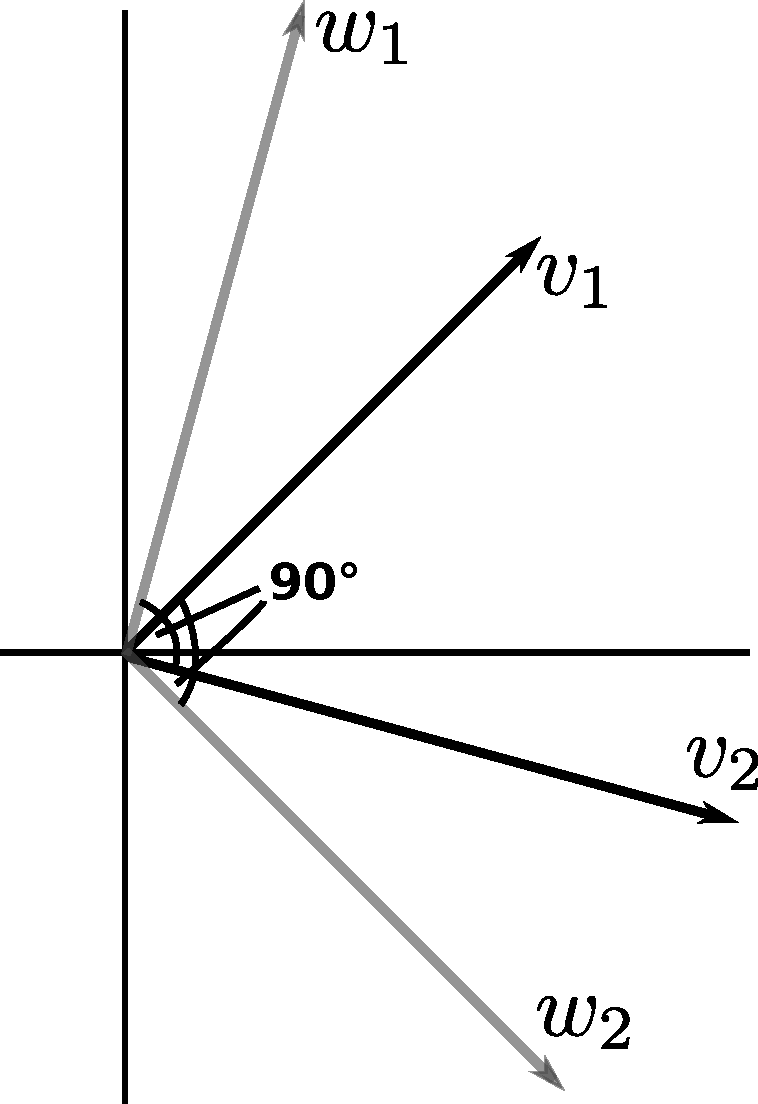
\includegraphics[width=0.3\linewidth]{chapters/3_solvers/3_2_iterative_solvers/figures/biorthogonal.pdf}
    \caption{Biorthogonal matrices $V$ and $W$ in the 2-dimensional case and $k=2$.}
    \label{fig:biorthogonal}
\end{figure}

\noindent The proof for the biorthogonal property is easily obtained from:
\begin{equation}
    WV=((Q^{-1})^T)^TQ = Q^{-1}Q = I
\end{equation}

\noindent From this, the biconjugate gradient (BiCG) method can be derived by using the Lanczos iteration to build a pair of biorthogonal bases for two subspaces:
\begin{equation}
\label{eqn:biconjugate_gradient}
    \begin{aligned}
    \mathcal{K}(A,v_1,k) &= \langle v_1, Av_1, \dots, A^{k-1}v_1\rangle \;\; \text{ and}\\
    \mathcal{L}(\transp{A},w_1,k) &= \langle w_1, Aw_1, \dots, A^{k-1}w_1 \rangle
    \end{aligned}
\end{equation}

\noindent At the $k$-th iteration, this method produces an iterate $\iter[k]{x}=\iter[0]{x}+V_k\iter[k]{y}$ with $\iter[k]{y} \in \real[k]$, which can be solved via:
\begin{equation}
    T_k\iter[k]{y}=W_k^T\iter[0]{r}
\end{equation}

\noindent The pseudo-code for this algorithm, which is basically a projection process on the subspaces defined in Equation~\hyperref[eqn:biconjugate_gradient]{\ref{eqn:biconjugate_gradient}} such that $\iter[k]{x} \in \mathcal{K}_k$ and $\iter[k]{r} \perp \mathcal{L}_k$ is provided in Algorithm~\hyperref[alg:biconjugate_gradient]{\ref{alg:biconjugate_gradient}}.

\begin{algorithm}[h]
  \caption{Biconjugate Gradient}
  \label{alg:biconjugate_gradient}
  \SetAlgoLined
  \DontPrintSemicolon
  \KwIn{matrix $A \in \mathbb{R}^{n \times n}$, vector $b \in \mathbb{R}^{n}$ and initial solution $\iter[0]{x} \in \mathbb{R}^{n}$}
  \KwOut{approximate solution $\iter[k]{x}$ to the system $Ax=b$\\
  \hrulealg}
  $\iter[0]{r} = b-A\iter[0]{x}$ \\
  choose $r^{(0)T}$ such that $\langle \iter[0]{r}; r^{(0)T}\rangle \neq 0$\\
  $\iter[0]{p} = \iter[0]{r}$ \\
  $p^{(i-1)T} = r^{(i-1)T}$ \\
  \For{$i = 1$ \KwTo $k$} {
    $\alpha = \langle \iter[i-1]{r};r^{(i-1)T} \rangle / \langle A\iter[i-1]{p};p^{(i-1)T} \rangle$ \\
    $\iter[i]{x} = \iter[i-1]{x}+\alpha \iter[i-1]{p}$ \\
    $\iter[i]{r} = \iter[i-1]{r} - \alpha A\iter[i-1]{p}$ \\
    $r^{(i-1)T} = p^{(i-1)T} -\alpha \transp{A} p^{(i-1)T}$ \\
    $\beta = \langle \iter[i]{r};r^{(i)T} \rangle / \langle \iter[i-1]{r};r^{(i-1)T} \rangle$ \\
    $\iter[i]{p} = \iter[i]{r} + \beta \iter[i-1]{p}$ \\
    $p^{(i)T} = r^{(i)T} + \beta p^{(i-1)T}$ \\
  }
\end{algorithm}

Compared to GMRES the algorithm has the big advantage that the vectors $q_{k+1}$ can be directly computed from the previous ones and as such there is no need to maintain the matrix $Q_k$. Consequently, the amount of work per iteration remains constant. As a drawback, the convergence of BiCG is generally slower and not monotonic, often exhibiting erratic behaviour. Therefore, a number of modifications have been proposed to smooth the convergence behaviour of the algorithm such as QMR (due to \cite{freund_qmr_1991}) and Bi-CGSTAB (due to \cite{van_der_vorst_bi-cgstab_1992}. Additional improvements include variants such as CGS (introduced in \cite{sonneveld_cgs_1989}) and TFQMR (proposed by \cite{freund_transpose-free_1994}, which avoid the need to multiply by $\transp{A}$ and thus are able to reduce the workload per iteration.

\subsubsection{Preconditioning}
\label{sec:preconditioning}
The convergence of any iterative solver is highly dependent on the properties of the matrix $A$ (e.g. eigenvalues, singular values, etc., depending on the solving technique). Preconditioning is a way to transforming the linear system in a way, such that these properties of the matrix are improved and faster convergence can be achieved. According to \cite{golub_matrix_2013}, any Krylov method used to solve the system $Ax=b$ will converge more rapidly if $A \in \realx{n}$ is "close to the identity matrix $I$". 
